\documentclass[../slides.tex]{subfiles}

\begin{document}

    \begin{frame}
        \tableofcontents[sections=\value{section}]
    \end{frame}
    
    \subsection{Tamaños de fuente}
    \begin{frame}{Tamaños de fuente}
        \begin{enumerate}
            \item \textbf{En todo el texto}: Se define en \texttt{\textbackslash documentclass[]\{\}}

            \item \textbf{En porciones del texto}:
                Comandos, ordenados de menor a mayor tamaño:
                \begin{enumerate}
                    \item \texttt{\textbackslash tiny}
                    \item \texttt{\textbackslash scriptsize}
                    \item \texttt{\textbackslash footnotesize}
                    \item \texttt{\textbackslash normalsize}
                    \item \texttt{\textbackslash large}
                    \item \texttt{\textbackslash Large}
                    \item \texttt{\textbackslash LARGE}
                    \item \texttt{\textbackslash huge}
                    \item \texttt{\textbackslash Huge}
                \end{enumerate}
                
        \end{enumerate}
    \end{frame}
    
    \begin{frame}{Tamaños de fuente}
        \begin{center}
            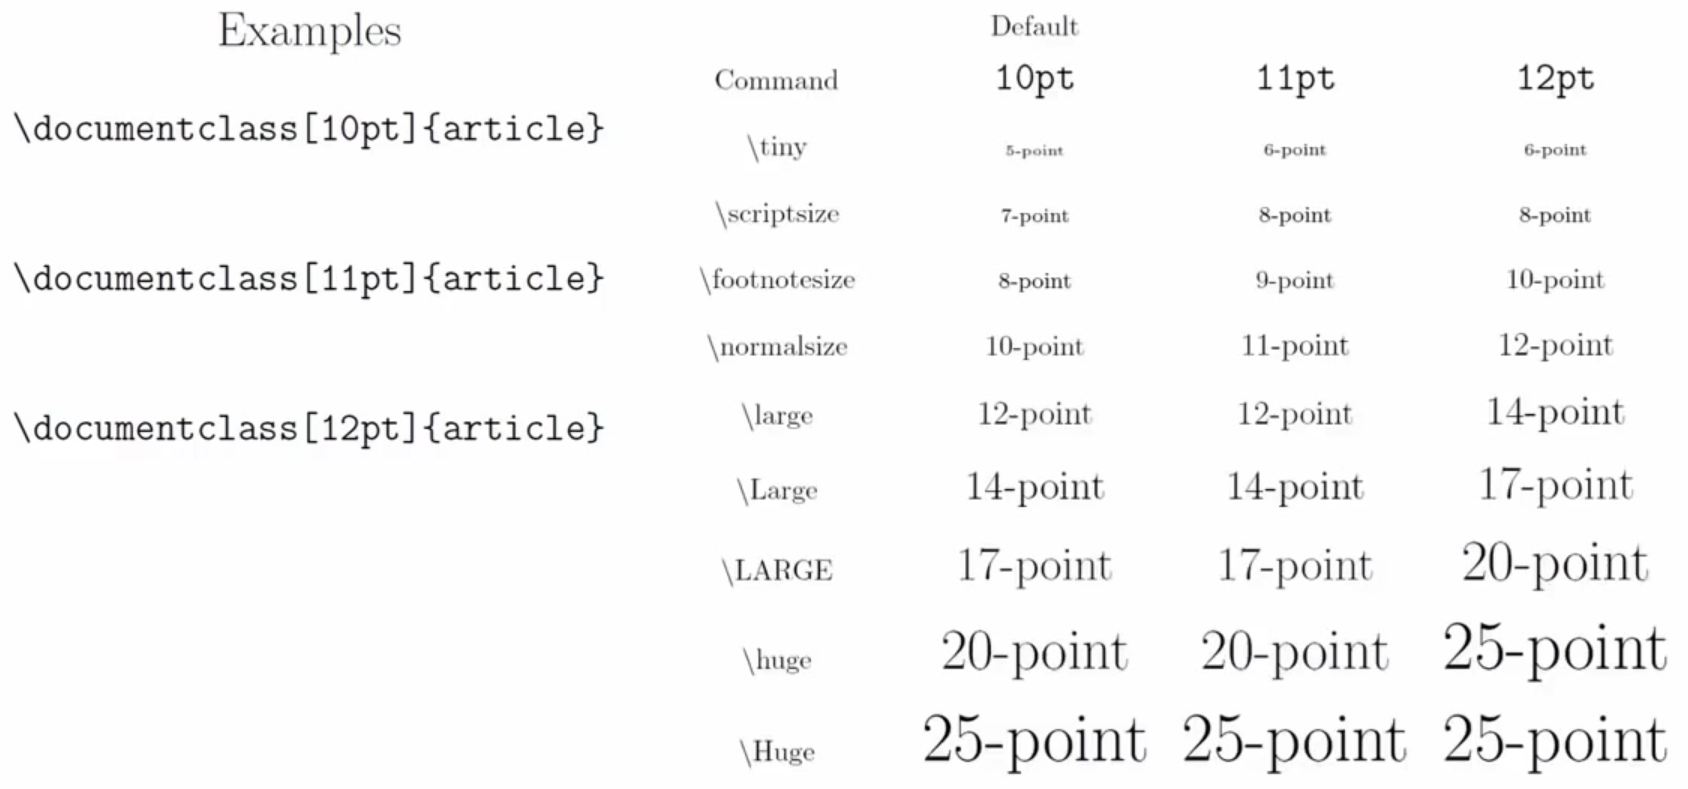
\includegraphics[scale=0.25]{sizes}
        \end{center}
    \end{frame}
    
    \subsection{Estilos de fuente}
    \begin{frame}{Estilos de fuente}
        En particular, tenemos tres herramientas usuales para dar estilo al texto presentado.
            \begin{enumerate}
                \item Negrita: \texttt{\textbackslash textbf} Este es un texto en \textbf{negrita}.
                    
                \item Cursiva: \texttt{\textbackslash textit} Este es un texto en \textit{cursiva}.
                \item Subrayado: \texttt{\textbackslash underline} Este es un texto \underline{subrayado}.
                \item Texto tipográfico: \texttt{\textbackslash texttt} Este es un texto \texttt{tipográfico}.
                \item Texto Small Caps: \texttt{\textbackslash textsc} Este es un texto \textsc{En Formato Sc., que consiste que las mínusculas son mayúsculas pero de un tamaño menor}.
            \end{enumerate}
    \end{frame}

    \subsection{Correcto uso de brackets}
    \begin{frame}[fragile]{Correcto uso de brackets}
\scriptsize{
        \begin{verbatim}
\textbf{\textit{\underline{Este es un texto en negritas, en cursiva y subrayado.}}}
        \end{verbatim}
        
        \begin{verbatim}
                           Este es un texto en negritas, en cursiva y subrayado.
                \underline{                                                     }
        \textit{                                                                 }
\textbf{                                                                          }
        \end{verbatim}
}
    \end{frame}
    
    \subsection{Listas}
    \begin{frame}[fragile]{Listas}
        \begin{enumerate}
            \item Lista enumerada:
                \begin{verbatim}
\begin{enumerate}
    \item Este es el primer item.
    \item Este es el segundo item.
\end{enumerate}
                \end{verbatim}
\begin{enumerate}
    \item Este es el primer item.
    \item Este es el segundo item.
\end{enumerate}
            \item Lista no enumerada:
                \begin{verbatim}
\begin{itemize}
    \item Este es el primer item.
    \item Este es el segundo item.
\end{itemize}
                \end{verbatim}
\begin{itemize}
    \item Este es el primer item.
    \item Este es el segundo item.
\end{itemize}
        \end{enumerate}
    \end{frame}
    
    \begin{frame}[fragile]{Listas}
        
    Se pueden personalizar los puntos de las enumeraciones. Por cada uno, se puede hacer
            \begin{verbatim}
\begin{enumerate}
    \item Este es el primer item.
    \item[A] Este es el segundo item.
    \item[5] Este es el tercer item.
\end{enumerate}
            \end{verbatim}
            \begin{enumerate}
                \item Este es el primer item.
                \item[A] Este es el segundo item.
                \item[5] Este es el tercer item.
            \end{enumerate}
    \begin{block}{}
    	El paquete \texttt{enumi} complementa las distintas opciones que se tienen para \texttt{enumerate}.
    \end{block}

    \end{frame}
    
    \subsection{Alineamiento de texto}
    \begin{frame}[fragile]{Alineamiento de texto}
        \begin{columns}
            \column{0.5\linewidth}
                \begin{verbatim}
Este texto no está centrado.
                \end{verbatim}
Este texto no está alineado.
            \column{0.5\linewidth}
                Texto centrado
                    \begin{verbatim}
\begin{center}
Este texto está centrado.
\end{center}
                    \end{verbatim}
\begin{center}
Este texto está centrado.
\end{center}
        \end{columns}
    \end{frame}

        \begin{frame}[fragile]{Alineamiento de texto}
        \begin{columns}
            \column{0.5\linewidth}
                Texto a la izquierda
                    \begin{verbatim}
\begin{flushleft}
Este texto está alineado a
la izquierda.
\end{flushleft}
                    \end{verbatim}
\begin{flushleft}
Este texto está alineado a la izquierda.
\end{flushleft}
            \column{0.5\linewidth}
                Texto a la derecha
                    \begin{verbatim}
\begin{flushright}
Este texto está alineado
a la derecha.
\end{flushright}
                    \end{verbatim}
\begin{flushright}
Este texto está alineado a la derecha.
\end{flushright}
        \end{columns}
    \end{frame}

    \subsection{Indentación en texto}
    
    \begin{frame}[fragile]{Párrafos}
        Para separar párrafos en un documento, se inserta una linea vacía entre uno y otro. Por ejemplo:
        \begin{verbatim}
Este es el primer párrafo que usaremos como ejemplo para 
observar como \LaTeX{} separa párrafos. Por si no se habia
dicho antes, el comando \LaTeX{} no genera el logo de LaTeX
en forma de texto.

Este es otro texto que usaremos como ejemplo, que consiste
en el segundo párrafo.
        \end{verbatim}
        \begin{block}{Nota}
        \LaTeX{} automáticamente indenta automaticamente nuevos párrafos. 
        \end{block}
    
    \end{frame}
    
    \begin{frame}{Indentación de un párrafo}
        \begin{alertblock}{Nota}
        La indentación dentro del código de \LaTeX{} es distinta a la indentación que aparece al final del documento.
        \end{alertblock}
        
        \begin{block}{Nota}
        Si deseamos especificamente no indentar un párrafo, se debe anteponer al párrafo el comando \texttt{\textbackslash noindent}.
        \end{block}
    \end{frame}

    \subsection{Saltos de linea}

    \begin{frame}[fragile]{Saltos de linea}
        Los saltos de linea se pueden realizar como
            \begin{verbatim}
Esta es la primera linea.\\
Esta es la segunda linea.\\[\baselineskip]
Esta es la tercera linea.\\[2\baselineskip]
Esta es la cuarta linea.
            \end{verbatim}
Esta es la primera linea.\\
Esta es la segunda linea.\\[\baselineskip]
Esta es la tercera linea.\\[2\baselineskip]
Esta es la cuarta linea.
    \end{frame}

    \subsection{Forzar nueva página}
    \begin{frame}{Forzar nueva página}
        Dos comandos:
            \begin{enumerate}
                \item \texttt{\textbackslash newpage}
                \item \texttt{\textbackslash clearpage}
            \end{enumerate}
        Ambos comandos se utilizan para saltar una nueva página. Poseen unas diferencias, las cuales se verán más adelante.
    \end{frame}
    
\end{document}
